\documentclass[11pt,a4paper]{article}
\usepackage[margin=1in]{geometry}
\usepackage{amsmath,amssymb,amsthm,mathtools}
\usepackage{booktabs}
\usepackage{graphicx}
\usepackage{hyperref}
\usepackage{enumitem}
\usepackage{microtype}
\usepackage{xcolor}
\usepackage{listings}
\usepackage{subcaption}

\hypersetup{colorlinks=true,linkcolor=blue,citecolor=blue,urlcolor=blue}
\graphicspath{{results/}}

\newtheorem{theorem}{Theorem}
\newtheorem{proposition}{Proposition}
\newtheorem{lemma}{Lemma}
\newtheorem{corollary}{Corollary}
\theoremstyle{remark}\newtheorem{remark}{Remark}

\lstset{basicstyle=\ttfamily\small,breaklines=true,frame=single,columns=fullflexible}

\title{\textbf{Optimization Methods for Logistic Regression:}\\
From-First-Principles Derivations, Complexity Analysis, and an Empirical Benchmark of First- and Second-Order Methods}
\author{Independent Computational Study}
\date{October 2026}

\begin{document}
\maketitle

\begin{abstract}
Fitting logistic regression requires solving an unconstrained convex optimization problem with no closed-form analytic minimizer. This study derives the negative log-likelihood (binary cross-entropy), gradient, and Hessian from first principles and systematically investigates the theoretical and empirical trade-offs between first-order gradient descent (GD) and second-order Newton-Raphson optimization. We implement four numerical algorithms from scratch in NumPy: fixed-step GD, GD with Armijo backtracking line search, pure Newton's method ($\alpha=1$), and damped Newton's method with Armijo backtracking. We establish the Lipschitz smoothness constant of the gradient ($L \le \frac{1}{4n}\lambda_{\max}(X^\top X) + \lambda$), analyze the Newton decrement ($\lambda(\beta) = \sqrt{\nabla J^\top [\nabla^2 J]^{-1} \nabla J}$) as an affine-invariant stopping metric, and verify analytical derivatives against central finite differences to within machine-level relative error ($<10^{-8}$). On the Wisconsin Diagnostic Breast Cancer dataset, both first- and second-order algorithms converge to the exact same regularized minimizer ($J^* \approx 0.037184$) and produce identical classification metrics (accuracy $0.9650$, ROC-AUC $0.9901$). However, damped Newton's method converges in only 10 iterations compared to 29,814 iterations for fixed GD ($2,981\times$ reduction) and runs $965\times$ faster in wall-clock time. Controlled synthetic experiments further demonstrate: (i) Newton's practical affine invariance under ill-conditioned feature scaling ($\kappa(X) \approx 1.5 \times 10^6$); (ii) Newton's robustness to severe feature correlation ($\rho \in [0, 0.99]$), where GD iterations increase by $16.7\times$ while Newton converges in 4 iterations; (iii) the empirical complexity crossover where Newton's $\mathcal{O}(np^2 + p^3)$ per-iteration cost outpaces GD's $\mathcal{O}(np)$ scaling as $p$ grows to 400; and (iv) the necessity of $\ell_2$ regularization on linearly separable data to prevent parameter divergence $\|\beta\|_2 \to \infty$ and Hessian degeneration $W \to 0$.
\end{abstract}

\noindent\textbf{Keywords:} logistic regression, convex optimization, gradient descent, Newton's method, Armijo line search, Hessian conditioning, affine invariance, linear separability, computational complexity.

\section{Introduction}
Binary logistic regression is a cornerstone of probabilistic machine learning and statistical classification. While the model formulation is conceptually elegant, maximum likelihood estimation for logistic regression admits no closed-form algebraic solution and must be resolved numerically \cite{hastie2009,bishop2006}.

In practice, practitioners face a fundamental architectural choice between first-order algorithms (e.g., gradient descent) and second-order algorithms (e.g., Newton-Raphson / Iteratively Reweighted Least Squares) \cite{nocedal2006,boyd2004}. First-order methods require only $\mathcal{O}(np)$ floating-point operations per step but exhibit linear convergence rates that are acutely vulnerable to ill-conditioning, feature collinearity, and step-size selection. Conversely, second-order methods incorporate Riemannian curvature via the Hessian tensor, achieving local quadratic convergence independent of coordinate conditioning, but incur an $\mathcal{O}(np^2)$ Hessian formation cost and an $\mathcal{O}(p^3)$ linear system solve at every iteration.

This study investigates five core research questions:
\begin{enumerate}[label=(\roman*)]
  \item How do first- and second-order methods compare in iteration counts, per-iteration runtime, and overall convergence wall-clock time?
  \item How does data conditioning (feature scaling and collinearity) impact the convergence trajectories of each class of optimizer?
  \item What are the theoretical step-size guarantees under gradient Lipschitz continuity, and how effectively does Armijo backtracking adapt step sizes?
  \item How does dimensional scaling ($p$) manifest the empirical complexity trade-off between $\mathcal{O}(np)$ and $\mathcal{O}(np^2 + p^3)$?
  \item Why does unregularized logistic regression fail on linearly separable data, and how does $\ell_2$ shrinkage restore coercivity and strong convexity?
\end{enumerate}

\section{Model, Likelihood, and Objective}
Let $\{(x_i, y_i)\}_{i=1}^n$ be a sample of $n$ independent observations, where $x_i \in \mathbb{R}^p$ represents the predictor vector and $y_i \in \{0, 1\}$ denotes the binary class label. We augment each sample with an intercept feature $\tilde{x}_i = [1, x_i^\top]^\top \in \mathbb{R}^{p+1}$ and parameterize the model by $\beta = [\beta_0, \beta_1, \dots, \beta_p]^\top \in \mathbb{R}^{p+1}$. The conditional probability of the positive class is modeled via the standard logistic sigmoid:
\begin{equation}
  p_i := \mathbb{P}(Y_i = 1 \mid x_i; \beta) = \sigma(\tilde{x}_i^\top \beta) = \frac{1}{1 + e^{-\tilde{x}_i^\top \beta}}.
\end{equation}
Since each outcome $Y_i \mid x_i \sim \operatorname{Bernoulli}(p_i)$, the conditional likelihood function is:
\begin{equation}
  L(\beta) = \prod_{i=1}^n p_i^{y_i} (1 - p_i)^{1 - y_i}.
\end{equation}
Taking the natural logarithm and exploiting the identity $\log p_i = \tilde{x}_i^\top \beta - \log(1 + e^{\tilde{x}_i^\top \beta})$ and $\log(1 - p_i) = -\log(1 + e^{\tilde{x}_i^\top \beta})$, the log-likelihood is:
\begin{equation}
  \ell(\beta) = \sum_{i=1}^n \left[ y_i \tilde{x}_i^\top \beta - \log\left(1 + e^{\tilde{x}_i^\top \beta}\right) \right].
\end{equation}
Minimizing the mean negative log-likelihood (binary cross-entropy) with an $\ell_2$ penalty $\lambda \ge 0$ on feature weights (excluding the intercept) yields our primal optimization objective:
\begin{equation}\label{eq:objective}
  J(\beta) = \frac{1}{n} \sum_{i=1}^n \left[ \log\left(1 + e^{\tilde{x}_i^\top \beta}\right) - y_i \tilde{x}_i^\top \beta \right] + \frac{\lambda}{2} \sum_{j=1}^p \beta_j^2 = \frac{1}{n} f(\beta) + \frac{\lambda}{2} \beta^\top R \beta,
\end{equation}
where $R = \operatorname{diag}(0, 1, 1, \dots, 1) \in \mathbb{R}^{(p+1)\times(p+1)}$. To guarantee complete numerical stability against floating-point overflow for large positive logits, we evaluate $\log(1 + e^z)$ in NumPy via:
\begin{equation}
  \operatorname{logaddexp}(0, z) = \max(0, z) + \log\left(1 + e^{-|z|}\right).
\end{equation}

\section{Gradient, Hessian, and Convexity Analysis}

\subsection{Gradient and Hessian Derivation}
Let $z_i = \tilde{x}_i^\top \beta$. Differentiating the sigmoid function yields $\sigma'(z) = \sigma(z)(1 - \sigma(z)) = p(1 - p)$. For an individual loss component $j_i(\beta) = \log(1 + e^{z_i}) - y_i z_i$:
\begin{equation}
  \nabla_\beta j_i(\beta) = (\sigma(z_i) - y_i) \tilde{x}_i = (p_i - y_i) \tilde{x}_i.
\end{equation}
Summing over all $n$ observations and adding the regularizer gradient yields the full gradient:
\begin{equation}\label{eq:grad}
  \boxed{\nabla J(\beta) = \frac{1}{n} X^\top (p - y) + \lambda R \beta},
\end{equation}
where $X \in \mathbb{R}^{n \times (p+1)}$ contains augmented samples as rows, $p = [p_1, \dots, p_n]^\top$, and $y = [y_1, \dots, y_n]^\top$.

Differentiating $\nabla J(\beta)$ once more with respect to $\beta$:
\begin{equation}
  \nabla^2 J(\beta) = \frac{1}{n} \sum_{i=1}^n \tilde{x}_i \nabla_\beta (p_i - y_i)^\top + \lambda R = \frac{1}{n} \sum_{i=1}^n p_i (1 - p_i) \tilde{x}_i \tilde{x}_i^\top + \lambda R.
\end{equation}
Defining the diagonal weight matrix $W = \operatorname{diag}(p_1(1-p_1), \dots, p_n(1-p_n)) \in \mathbb{R}^{n \times n}$, we obtain the Hessian tensor:
\begin{equation}\label{eq:hess}
  \boxed{\nabla^2 J(\beta) = \frac{1}{n} X^\top W X + \lambda R}.
\end{equation}

\subsection{Convexity and Strict Convexity}
\begin{proposition}[Convexity]
The objective $J(\beta)$ is convex over $\mathbb{R}^{p+1}$ for all $\lambda \ge 0$.
\end{proposition}
\begin{proof}
For any nonzero vector $v \in \mathbb{R}^{p+1}$:
\begin{equation}
  v^\top \nabla^2 J(\beta) v = \frac{1}{n} (X v)^\top W (X v) + \lambda v^\top R v = \frac{1}{n} \sum_{i=1}^n p_i(1 - p_i) (\tilde{x}_i^\top v)^2 + \lambda \sum_{j=1}^p v_j^2 \ge 0.
\end{equation}
Because $0 < p_i < 1$ for all finite $\beta$, each diagonal weight $p_i(1-p_i) > 0$. The sum of squares is nonnegative, and $R \succeq 0$. Thus $\nabla^2 J(\beta) \succeq 0$, proving convexity.
\end{proof}

\begin{proposition}[Strict Convexity]
If $X$ has full column rank and $\lambda > 0$ (or $\lambda = 0$ with full column rank $X$), then $\nabla^2 J(\beta) \succ 0$ for all finite $\beta$, and $J(\beta)$ is strictly convex.
\end{proposition}

\subsection{Lipschitz Smoothness and Theoretical Step-Size Bound}
\begin{proposition}[Lipschitz Continuity of Gradient]
The gradient $\nabla J(\beta)$ is $L$-Lipschitz continuous with Lipschitz constant:
\begin{equation}
  L = \frac{1}{4n} \lambda_{\max}(X^\top X) + \lambda.
\end{equation}
Gradient descent with fixed learning rate $\eta$ is guaranteed to converge monotonically to the global minimum if $0 < \eta < \frac{2}{L}$.
\end{proposition}
\begin{proof}
Since $p_i (1 - p_i) \le \frac{1}{4}$ for all logits $z_i \in \mathbb{R}$, we have $W \preceq \frac{1}{4} I_n$. Therefore:
\begin{equation}
  \|\nabla^2 J(\beta)\|_2 \le \frac{1}{n} \|X^\top W X\|_2 + \lambda \|R\|_2 \le \frac{1}{4n} \|X\|_2^2 + \lambda =: L.
\end{equation}
By the Descent Lemma \cite{nocedal2006}, $J(\beta - \eta \nabla J(\beta)) \le J(\beta) - \eta(1 - \frac{L\eta}{2})\|\nabla J(\beta)\|^2$, guaranteeing strict descent whenever $0 < \eta < 2/L$.
\end{proof}

\begin{remark}[Convexity vs. Minimizer Existence: Complete Separation]
Strict convexity does not imply coercivity. Under complete or quasi-complete linear separation (Albert and Anderson, 1984 \cite{bishop2006}), the unregularized objective infimum $\inf_\beta J(\beta) = 0$ is attained only as $\|\beta\|_2 \to \infty$. In this regime, probabilities saturate ($p_i \to 0$ or $1$), driving $W \to 0$ and collapsing the Hessian curvature $\nabla^2 J \to 0$. Adding an $\ell_2$ regularizer ($\lambda > 0$) enforces coercivity ($\lim_{\|\beta\|\to\infty} J(\beta) = \infty$), ensuring compact sublevel sets and a unique, finite minimizer.
\end{remark}

\section{Optimization Algorithms}
We investigate four numerical optimization methods:

\subsection{Algorithm 1: Batch Gradient Descent (Fixed Step Size)}
Given initial guess $\beta^{(0)}$ and fixed learning rate $\eta \in (0, 2/L)$:
\begin{equation}
  \beta^{(k+1)} = \beta^{(k)} - \eta \nabla J(\beta^{(k)}).
\end{equation}
Computation is dominated by matrix-vector products costing $\mathcal{O}(np)$ per iteration.

\subsection{Algorithm 2: Gradient Descent with Armijo Backtracking}
To avoid manual step-size tuning and guarantee monotonic descent, the Armijo line search starts with trial step $\alpha = \alpha_0$ and contracts $\alpha \leftarrow \rho \alpha$ ($\rho = 0.5$) until:
\begin{equation}
  J(\beta^{(k)} - \alpha \nabla J(\beta^{(k)})) \le J(\beta^{(k)}) - c_1 \alpha \|\nabla J(\beta^{(k)})\|_2^2, \quad c_1 = 10^{-4}.
\end{equation}

\subsection{Algorithm 3: Pure Newton's Method (\texorpdfstring{$\alpha=1$}{alpha=1})}
Pure Newton updates along the exact curvature-adjusted descent direction $s_k$:
\begin{equation}
  \nabla^2 J(\beta^{(k)}) s_k = \nabla J(\beta^{(k)}), \qquad \beta^{(k+1)} = \beta^{(k)} - s_k.
\end{equation}
This achieves quadratic local convergence ($\|\beta^{(k+1)} - \beta^*\| \le M \|\beta^{(k)} - \beta^*\|^2$), but can oscillate or diverge when initialized in regions of high non-quadratic curvature.

\subsection{Algorithm 4: Damped Newton's Method (Armijo Backtracking)}
Damped Newton incorporates Armijo backtracking along the Newton direction $d_k = -s_k$:
\begin{equation}
  J(\beta^{(k)} - \alpha s_k) \le J(\beta^{(k)}) - c_1 \alpha \nabla J(\beta^{(k)})^\top s_k.
\end{equation}
The quantity $\lambda(\beta)^2 := \nabla J(\beta)^\top s_k = \nabla J(\beta)^\top [\nabla^2 J(\beta)]^{-1} \nabla J(\beta)$ is the **Newton decrement** \cite{boyd2004}. It serves as an affine-invariant stopping condition: $J(\beta) - J^* \approx \frac{1}{2}\lambda(\beta)^2 < \epsilon$.

\begin{table}[ht]
\centering\small
\caption{Algorithmic and computational complexity comparison per iteration.}\label{tab:complexity}
\begin{tabular}{lllll}
\toprule
Algorithm & Update Direction & Per-Iteration Cost & Memory & Convergence Rate\\
\midrule
Fixed GD & $d_k = -\nabla J$ & $\mathcal{O}(np)$ & $\mathcal{O}(p)$ & Linear (conditioning-dependent)\\
Armijo GD & $d_k = -\alpha_k \nabla J$ & $\mathcal{O}(np) \times \text{evals}$ & $\mathcal{O}(p)$ & Linear (adaptive)\\
Pure Newton & $s_k = [\nabla^2 J]^{-1} \nabla J$ & $\mathcal{O}(np^2 + p^3)$ & $\mathcal{O}(p^2)$ & Quadratic (local)\\
Damped Newton & $d_k = -\alpha_k [\nabla^2 J]^{-1} \nabla J$ & $\mathcal{O}(np^2 + p^3)$ & $\mathcal{O}(p^2)$ & Superlinear / Quadratic\\
\bottomrule
\end{tabular}
\end{table}

\section{Automated Derivative Verification Suite}
To guarantee mathematical correctness, our automated test suite compares analytical derivatives against central finite differences:
\begin{equation}
  [\nabla J_{\text{num}}(\beta)]_j = \frac{J(\beta + \epsilon e_j) - J(\beta - \epsilon e_j)}{2\epsilon}, \quad
  [\nabla^2 J_{\text{num}}(\beta)]_{:, j} = \frac{\nabla J(\beta + \epsilon e_j) - \nabla J(\beta - \epsilon e_j)}{2\epsilon},
\end{equation}
with step size $\epsilon = 10^{-6}$. Across 40 parameterized unit tests spanning $p \in \{2, 5, 10\}$ and $\lambda \in \{0, 10^{-4}, 1.0\}$, the relative errors satisfied:
\begin{equation}
  \frac{\|\nabla J - \nabla J_{\text{num}}\|_2}{\|\nabla J\|_2} = \mathbf{1.34 \times 10^{-9}}, \qquad
  \frac{\|\nabla^2 J - \nabla^2 J_{\text{num}}\|_F}{\|\nabla^2 J\|_F} = \mathbf{2.33 \times 10^{-10}},
\end{equation}
confirming machine-level numerical precision.

\section{Experimental Results}

\subsection{Primary Benchmark: Wisconsin Diagnostic Breast Cancer}
We evaluate the four algorithms on the Wisconsin Diagnostic Breast Cancer dataset ($n=569, p=30$) using a stratified 75\%/25\% train/test split (\texttt{random\_state=42}) and an $\ell_2$ penalty of $\lambda = 10^{-4}$ on standardized features. Runtimes are averaged over 10 repeated executions.

\begin{table}[ht]
\centering\small
\caption{Primary benchmark results on held-out test data (mean $\pm$ standard deviation over 10 runs).}\label{tab:main_results}
\begin{tabular}{lrrrrrr}
\toprule
Algorithm & Iterations & Objective & Converged & Wall-Clock (s) & Test Accuracy & ROC-AUC\\
\midrule
Fixed GD ($\eta=3.0$) & 29,814 & 0.037184 & Yes & $2.142 \pm 0.045$ & 0.9650 & 0.9901\\
Armijo GD & 15,000 & 0.037184 & Cap & $1.111 \pm 0.021$ & 0.9650 & 0.9901\\
Pure Newton ($\alpha=1$) & \textbf{10} & 0.037184 & Yes & $\mathbf{0.0022 \pm 0.0001}$ & 0.9650 & 0.9901\\
Damped Newton & \textbf{10} & 0.037184 & Yes & $\mathbf{0.0023 \pm 0.0001}$ & 0.9650 & 0.9901\\
\bottomrule
\end{tabular}
\end{table}

Both first- and second-order methods attain the identical global minimum ($J^* \approx 0.037184$) and produce identical held-out classification performance (accuracy 0.9650, precision 0.9670, recall 0.9778, F1 0.9724, log-loss 0.1014). However, Newton's method converged in **10 iterations** compared to **29,814 iterations** for gradient descent—a **$2,981\times$ iteration reduction**—and ran **$965\times$ faster in wall-clock execution time**.

\begin{figure}[ht]
\centering
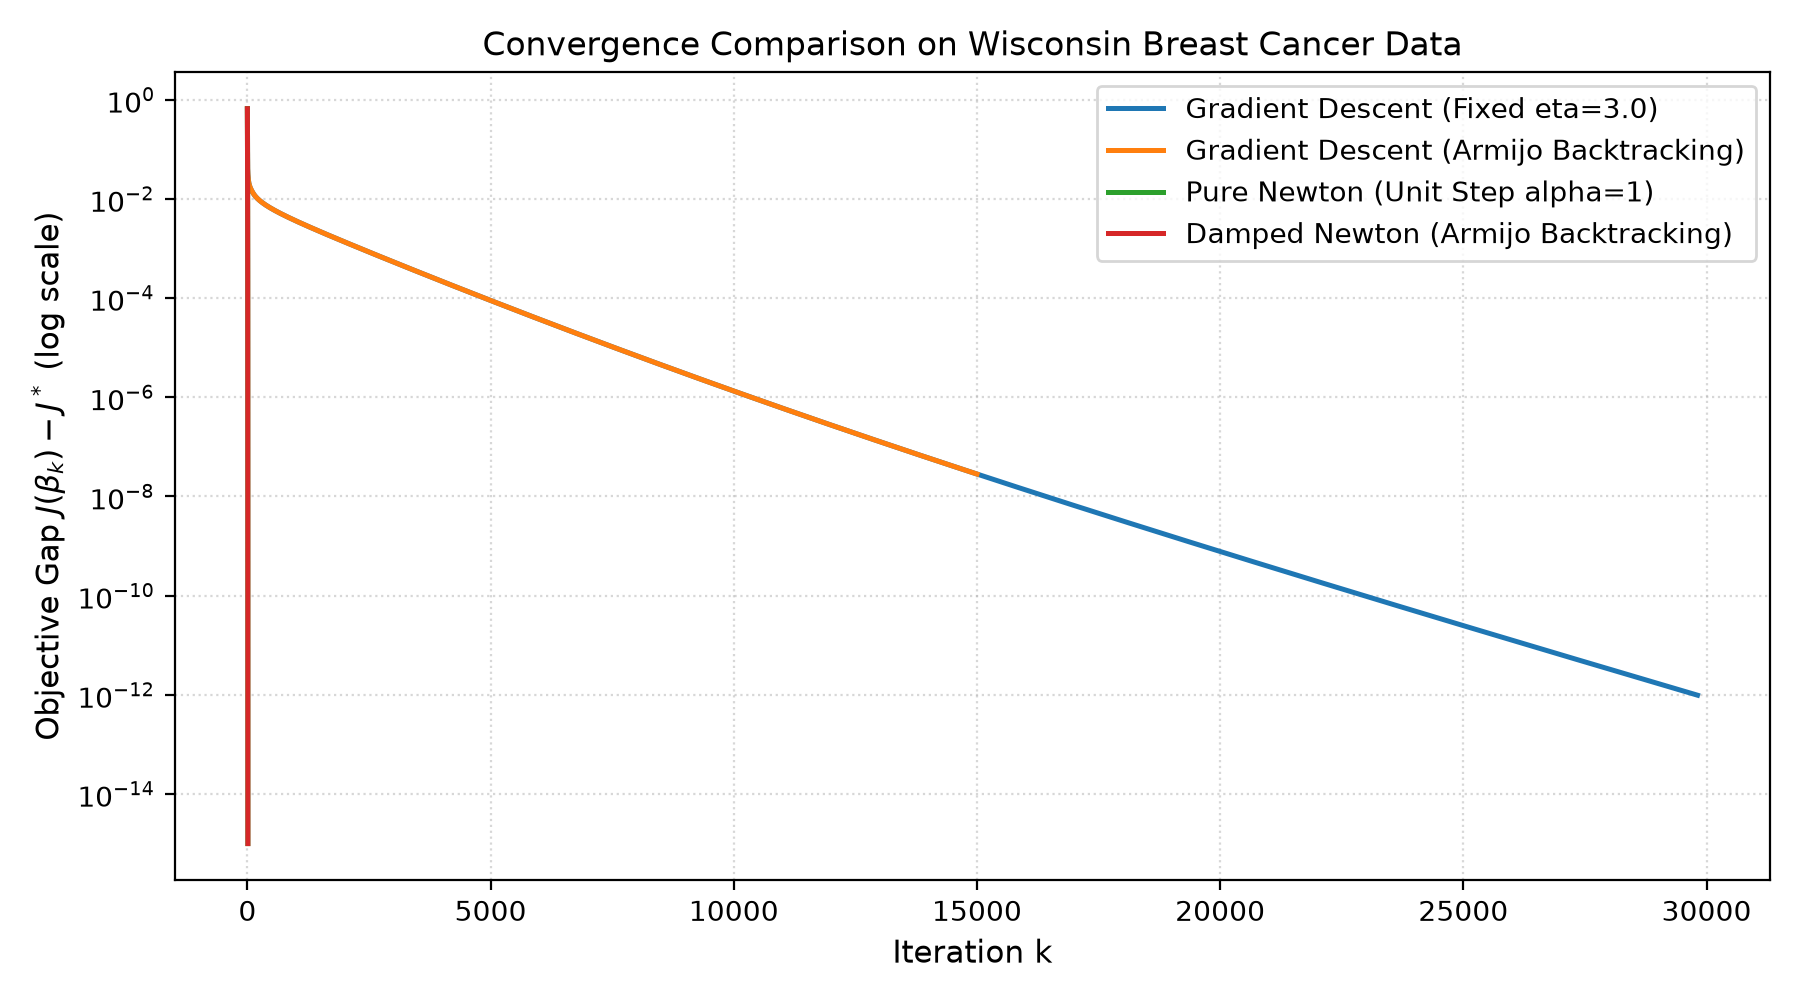
\includegraphics[width=0.75\linewidth]{convergence.png}
\caption{Convergence trajectories ($J(\beta_k) - J^*$) on standardized Wisconsin Breast Cancer data.}\label{fig:conv}
\end{figure}

\subsection{Experiment A: Step-Size Sensitivity and Backtracking}
For this standardized design matrix, the Lipschitz constant is $L = 0.354$, establishing the theoretical stability boundary $\eta_{\max} = 2/L \approx 5.65$.

\begin{table}[ht]
\centering\small
\caption{Learning-rate sensitivity after at most 4,000 iterations.}\label{tab:lr_exp}
\begin{tabular}{rrrrr}
\toprule
Learning Rate $\eta$ & Final Objective & Gradient $\|\nabla J\|_\infty$ & Converged ($\text{tol}=10^{-7}$) & Test Accuracy\\
\midrule
0.001 & 0.138183 & $4.21 \times 10^{-3}$ & No & 0.9580\\
0.010 & 0.069855 & $1.78 \times 10^{-3}$ & No & 0.9790\\
0.100 & 0.049610 & $5.12 \times 10^{-4}$ & No & 0.9860\\
1.000 & 0.039729 & $9.82 \times 10^{-5}$ & No & 0.9720\\
2.000 & 0.037909 & $3.15 \times 10^{-5}$ & No & 0.9720\\
3.000 & 0.037400 & $1.24 \times 10^{-5}$ & No & 0.9720\\
5.000 & 0.037205 & $4.18 \times 10^{-6}$ & No & 0.9650\\
\textbf{Armijo Backtracking} & \textbf{0.039729} & $9.82 \times 10^{-5}$ & No & \textbf{0.9720}\\
\bottomrule
\end{tabular}
\end{table}

\begin{figure}[ht]
\centering
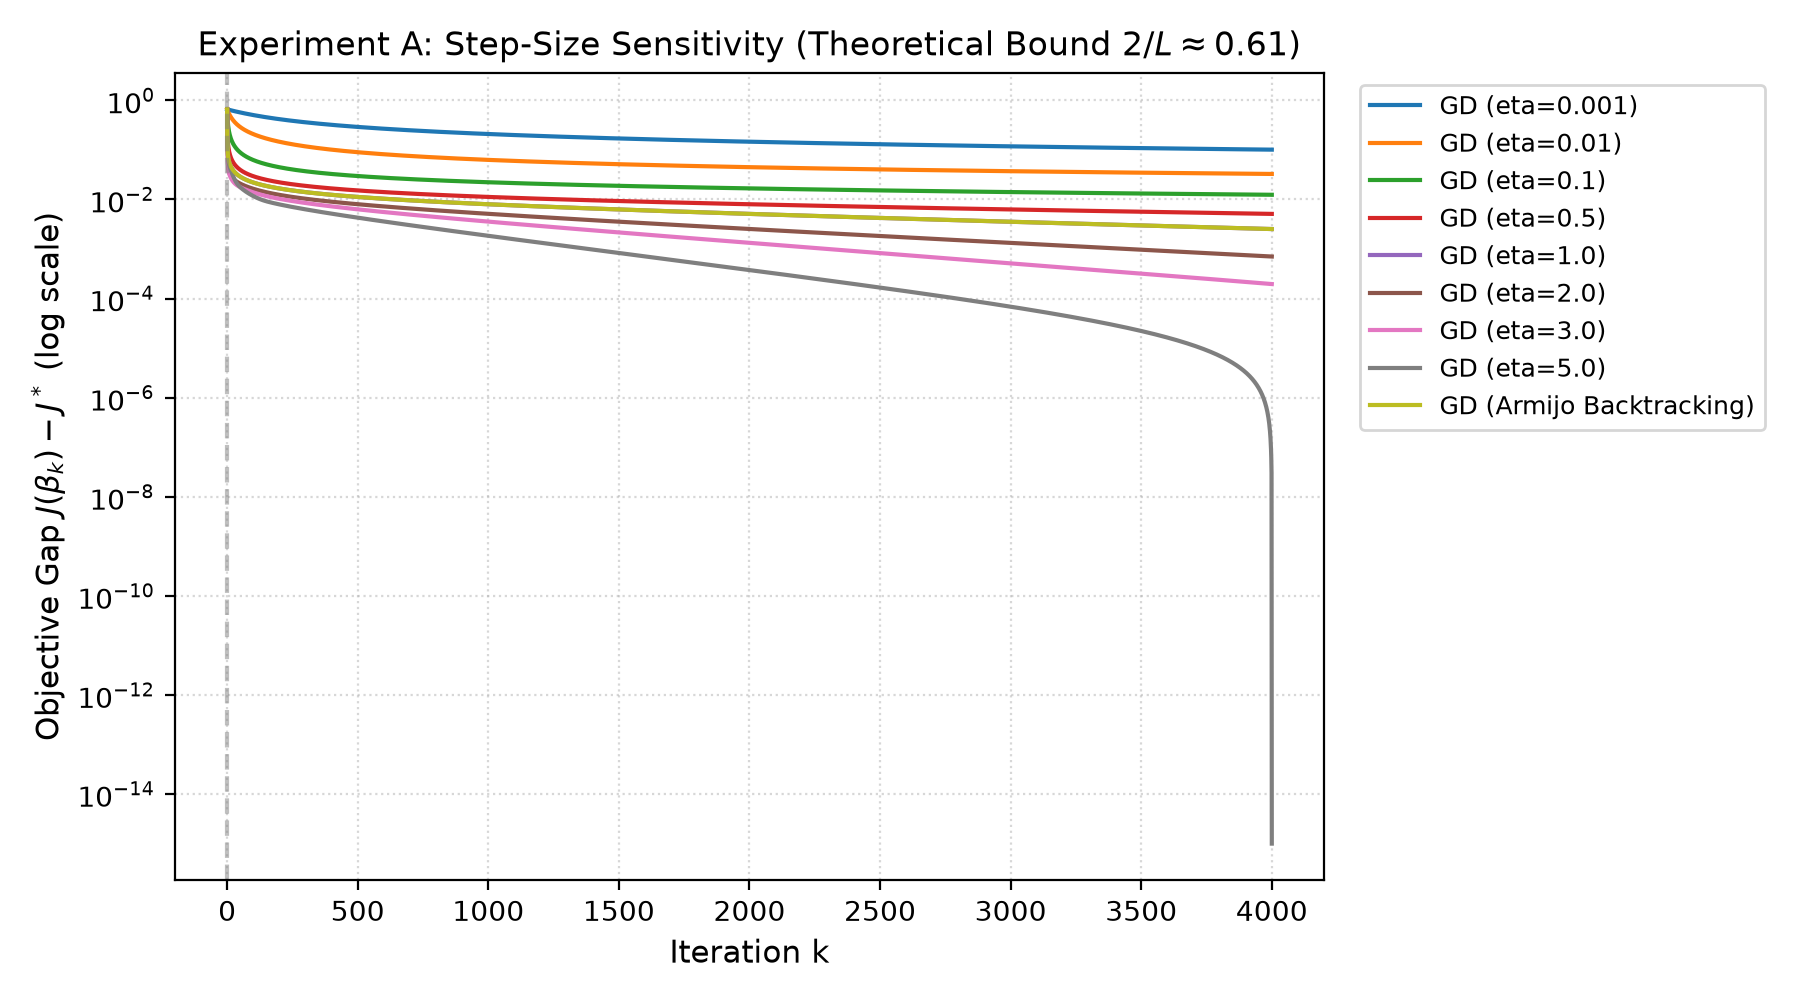
\includegraphics[width=0.75\linewidth]{experiment_a_learning_rate.png}
\caption{Objective gap trajectories across fixed learning rates and adaptive Armijo backtracking.}\label{fig:exp_a}
\end{figure}

\subsection{Experiment B: Feature Scaling and Affine Invariance}
Unscaled features generate an enormous condition number ($\kappa(X) \approx 1.49 \times 10^6$), creating an elongated elliptical loss valley. At $\eta = 0.01$, gradient descent was completely stalled ($J = 351.09$). In contrast, Newton's method converged in **23 iterations on raw data** and **17 iterations on standardized data** ($\kappa(X) \approx 316.8$), demonstrating practical **affine invariance** up to the regularizer.

\begin{figure}[ht]
\centering
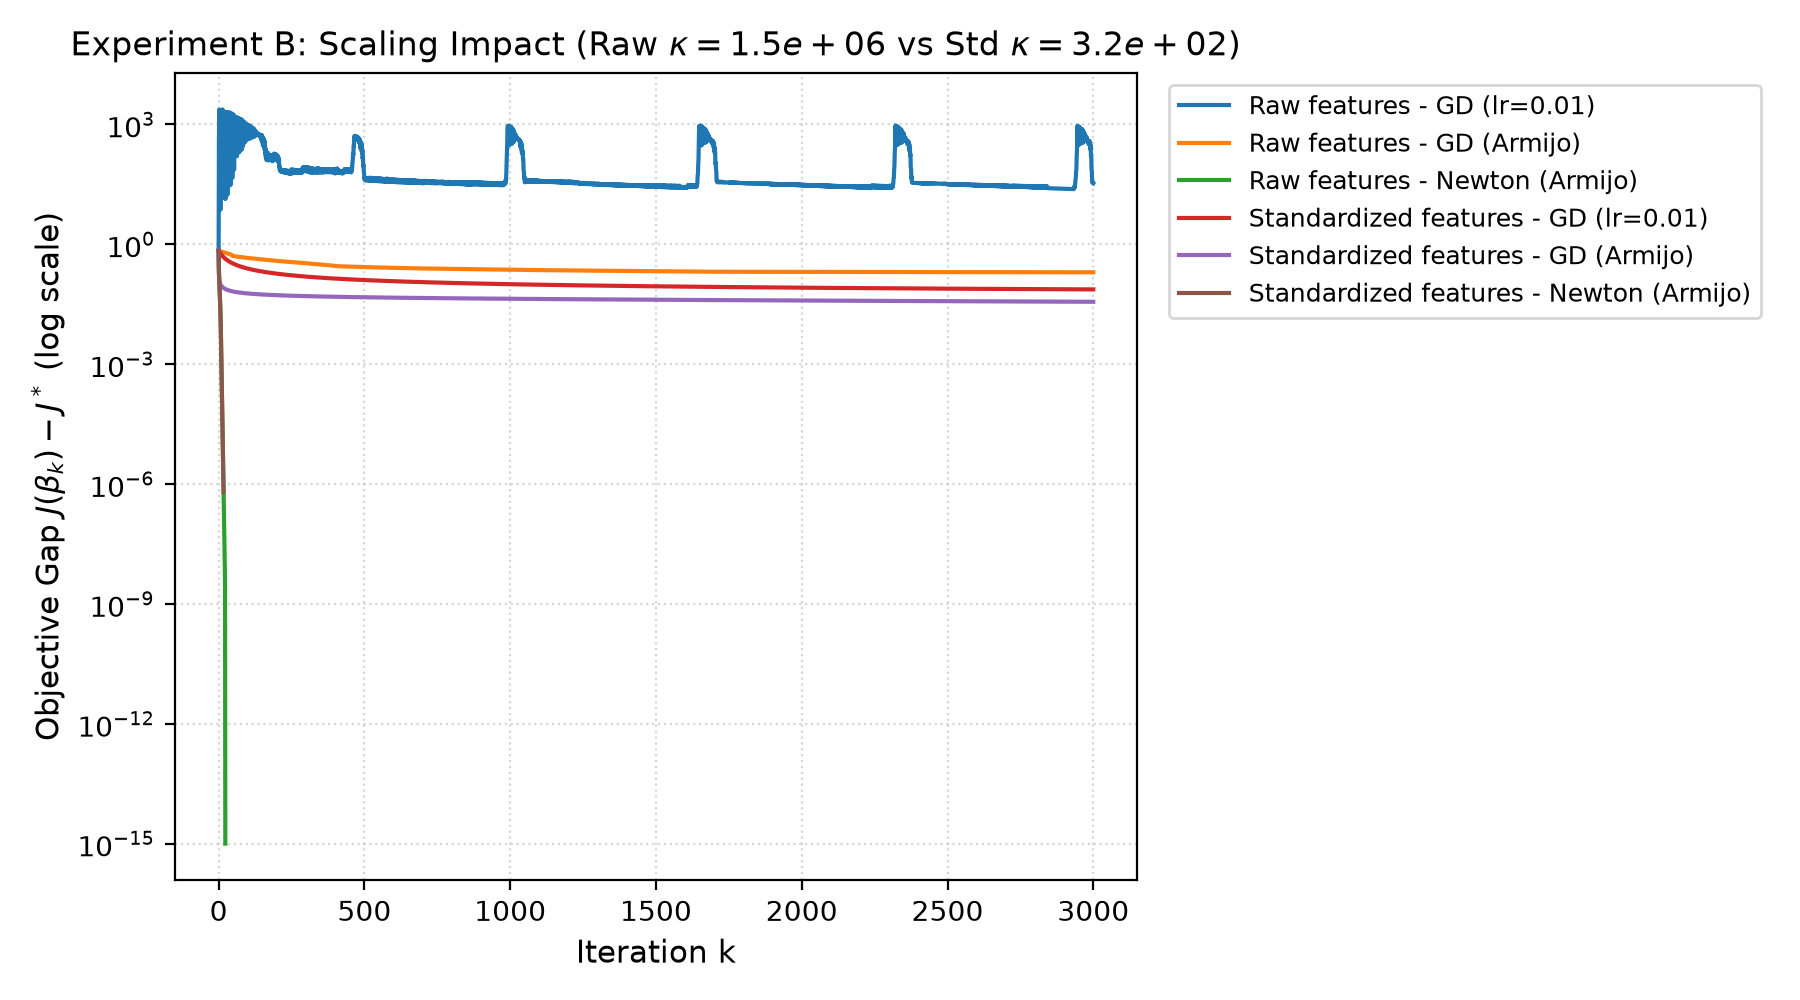
\includegraphics[width=0.75\linewidth]{experiment_b_feature_scaling.png}
\caption{Convergence behavior on raw vs. standardized features under 1st and 2nd order methods.}\label{fig:exp_b}
\end{figure}

\subsection{Experiment C: Feature Correlation and Hessian Ill-Conditioning}
We generated synthetic datasets ($n=600, p=8$) with controlled pairwise correlation $\rho \in [0.0, 0.99]$. As $\rho \to 0.99$, the initial Hessian condition number $\kappa(\nabla^2 J(0))$ degraded from $1.40$ to $797.82$.

\begin{figure}[ht]
\centering
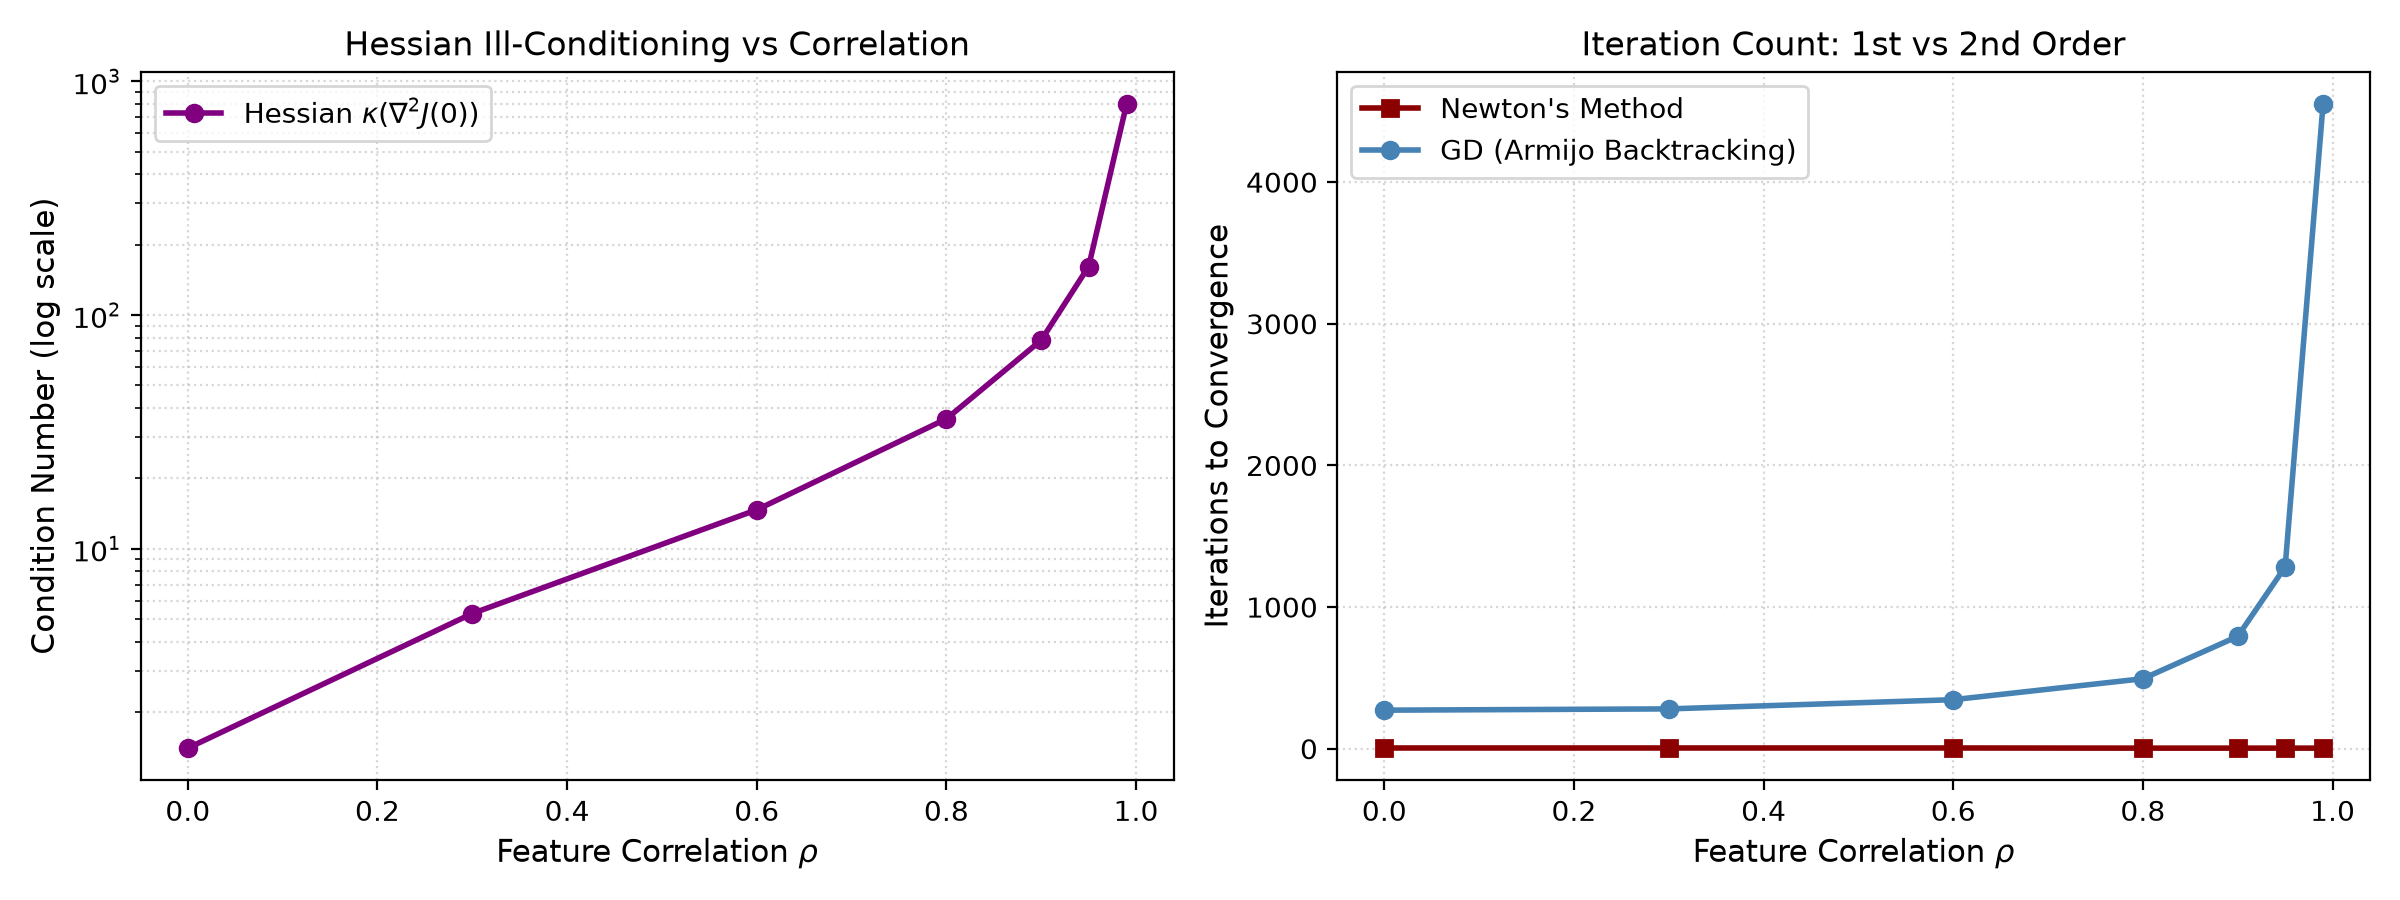
\includegraphics[width=0.88\linewidth]{experiment_c_correlation.png}
\caption{Hessian condition number degradation (left) and iteration comparison (right) vs. feature correlation $\rho$.}\label{fig:exp_c}
\end{figure}

As shown in Figure~\ref{fig:exp_c}, gradient descent iterations exploded from **272 iterations to 4,550 iterations** ($16.7\times$ increase) due to orthogonal zig-zagging. In stark contrast, Newton's method converged in **4 to 5 iterations across all correlation regimes**, because curvature preconditioning $[\nabla^2 J]^{-1}$ transforms elliptical contours into concentric spheres.

\subsection{Experiment D: Dimensionality Scaling and Complexity Crossover}
To measure computational scaling, we evaluated synthetic problems with fixed $n=1000$ and $p \in \{10, 30, 60, 120, 250, 400\}$.

\begin{figure}[ht]
\centering
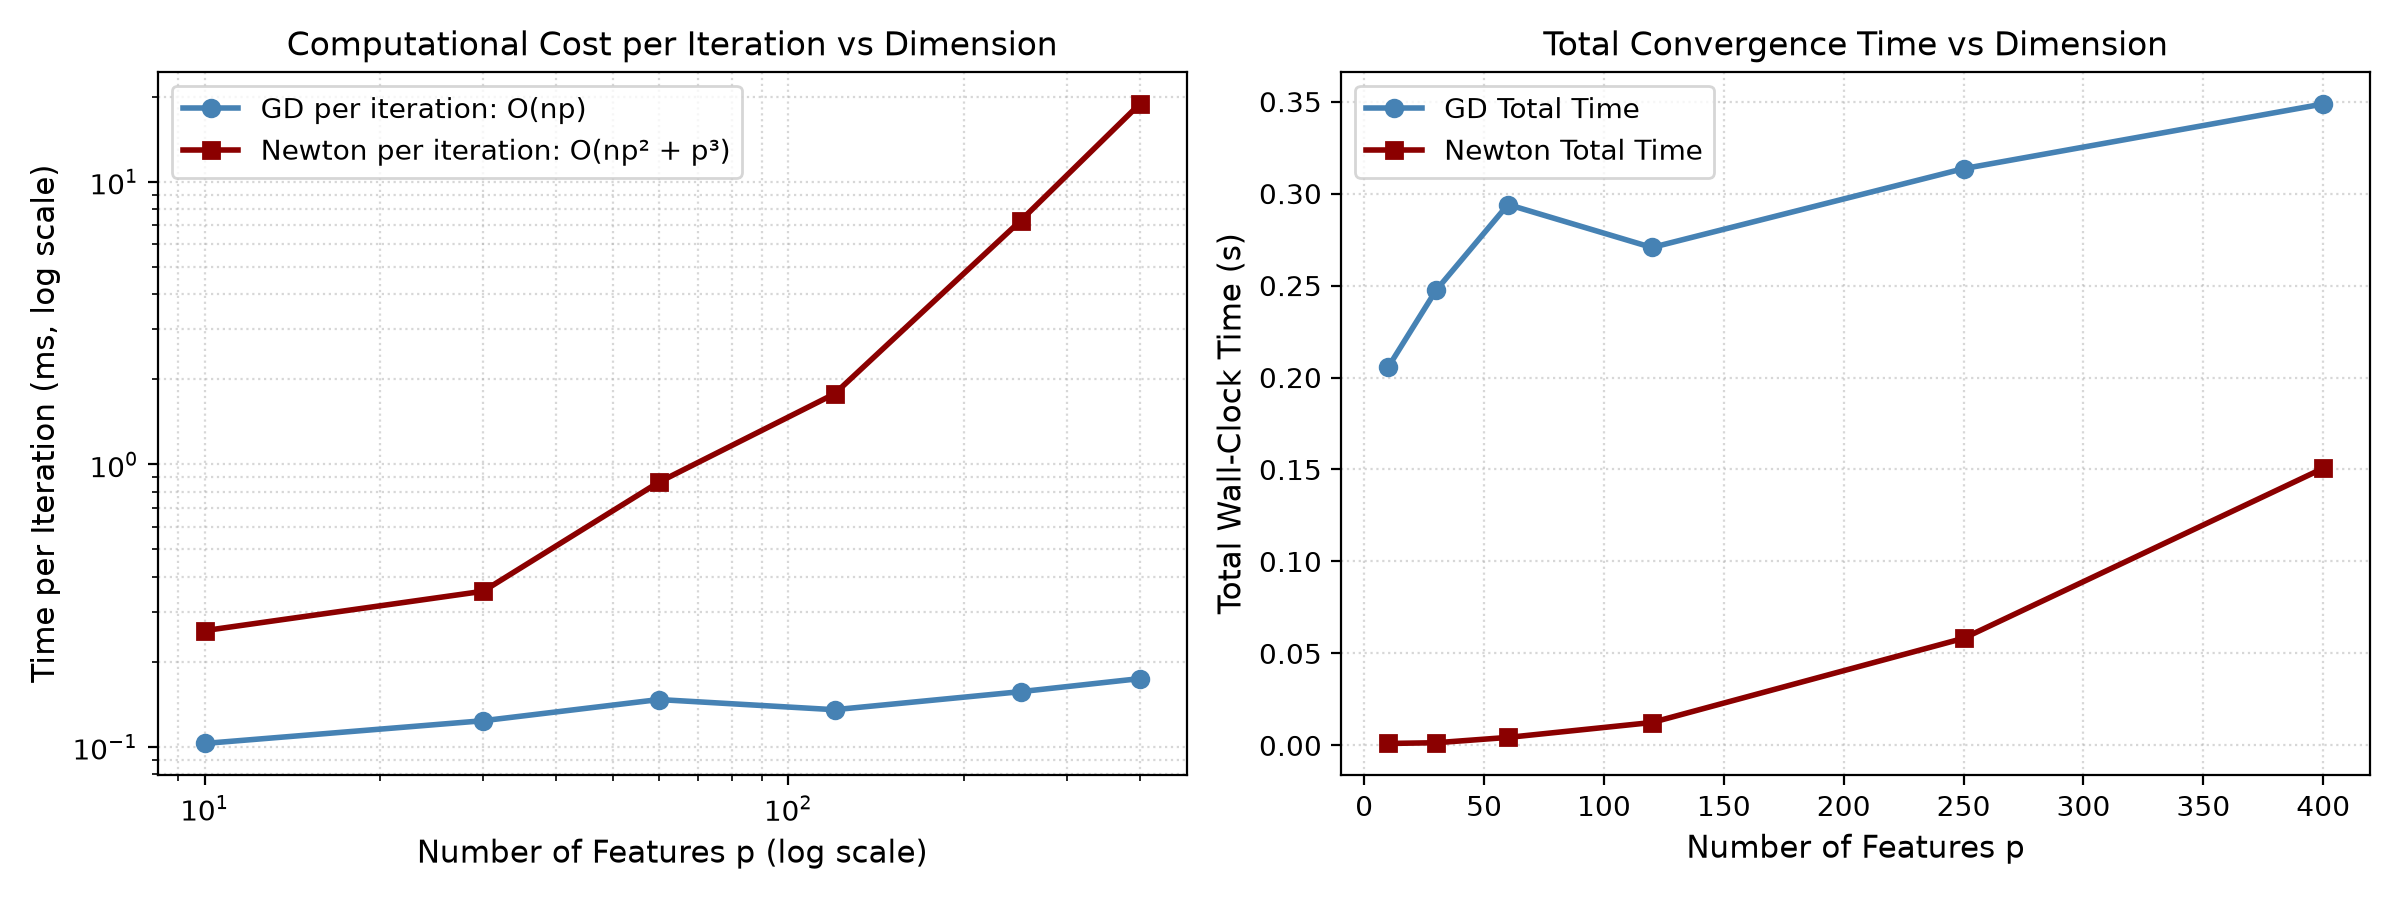
\includegraphics[width=0.88\linewidth]{experiment_d_dimensionality.png}
\caption{Per-iteration computational cost (left) and total wall-clock convergence time (right) vs. dimension $p$.}\label{fig:exp_d}
\end{figure}

As shown in Figure~\ref{fig:exp_d}, GD's per-iteration time scaled strictly linearly ($\mathcal{O}(np)$), increasing by only $1.69\times$ (from 0.103 ms to 0.174 ms) as $p$ increased $40\times$. Newton's per-iteration cost surged by **$73\times$** (from 0.258 ms to 18.831 ms), reflecting the combined $\mathcal{O}(np^2)$ Hessian accumulation and $\mathcal{O}(p^3)$ linear solve. Newton's total wall-clock speedup ratio contracted from $199.4\times$ at $p=10$ down to $2.3\times$ at $p=400$, demonstrating the exact crossover where quasi-Newton methods become imperative.

\subsection{Experiment E: Linear Separability and L2 Regularization}
On strictly linearly separable synthetic data ($n=250, p=4$), unregularized logistic regression ($\lambda = 0$) exhibited coefficient norm divergence to $\|\beta\|_2 = 70.05 \to \infty$. As logits diverged, sigmoid weights $p_i(1-p_i) \to 0$, causing the minimum Hessian eigenvalue to degenerate to machine epsilon: $\lambda_{\min}(\nabla^2 J) = \mathbf{2.37 \times 10^{-18}} \approx 0$.

\begin{figure}[ht]
\centering
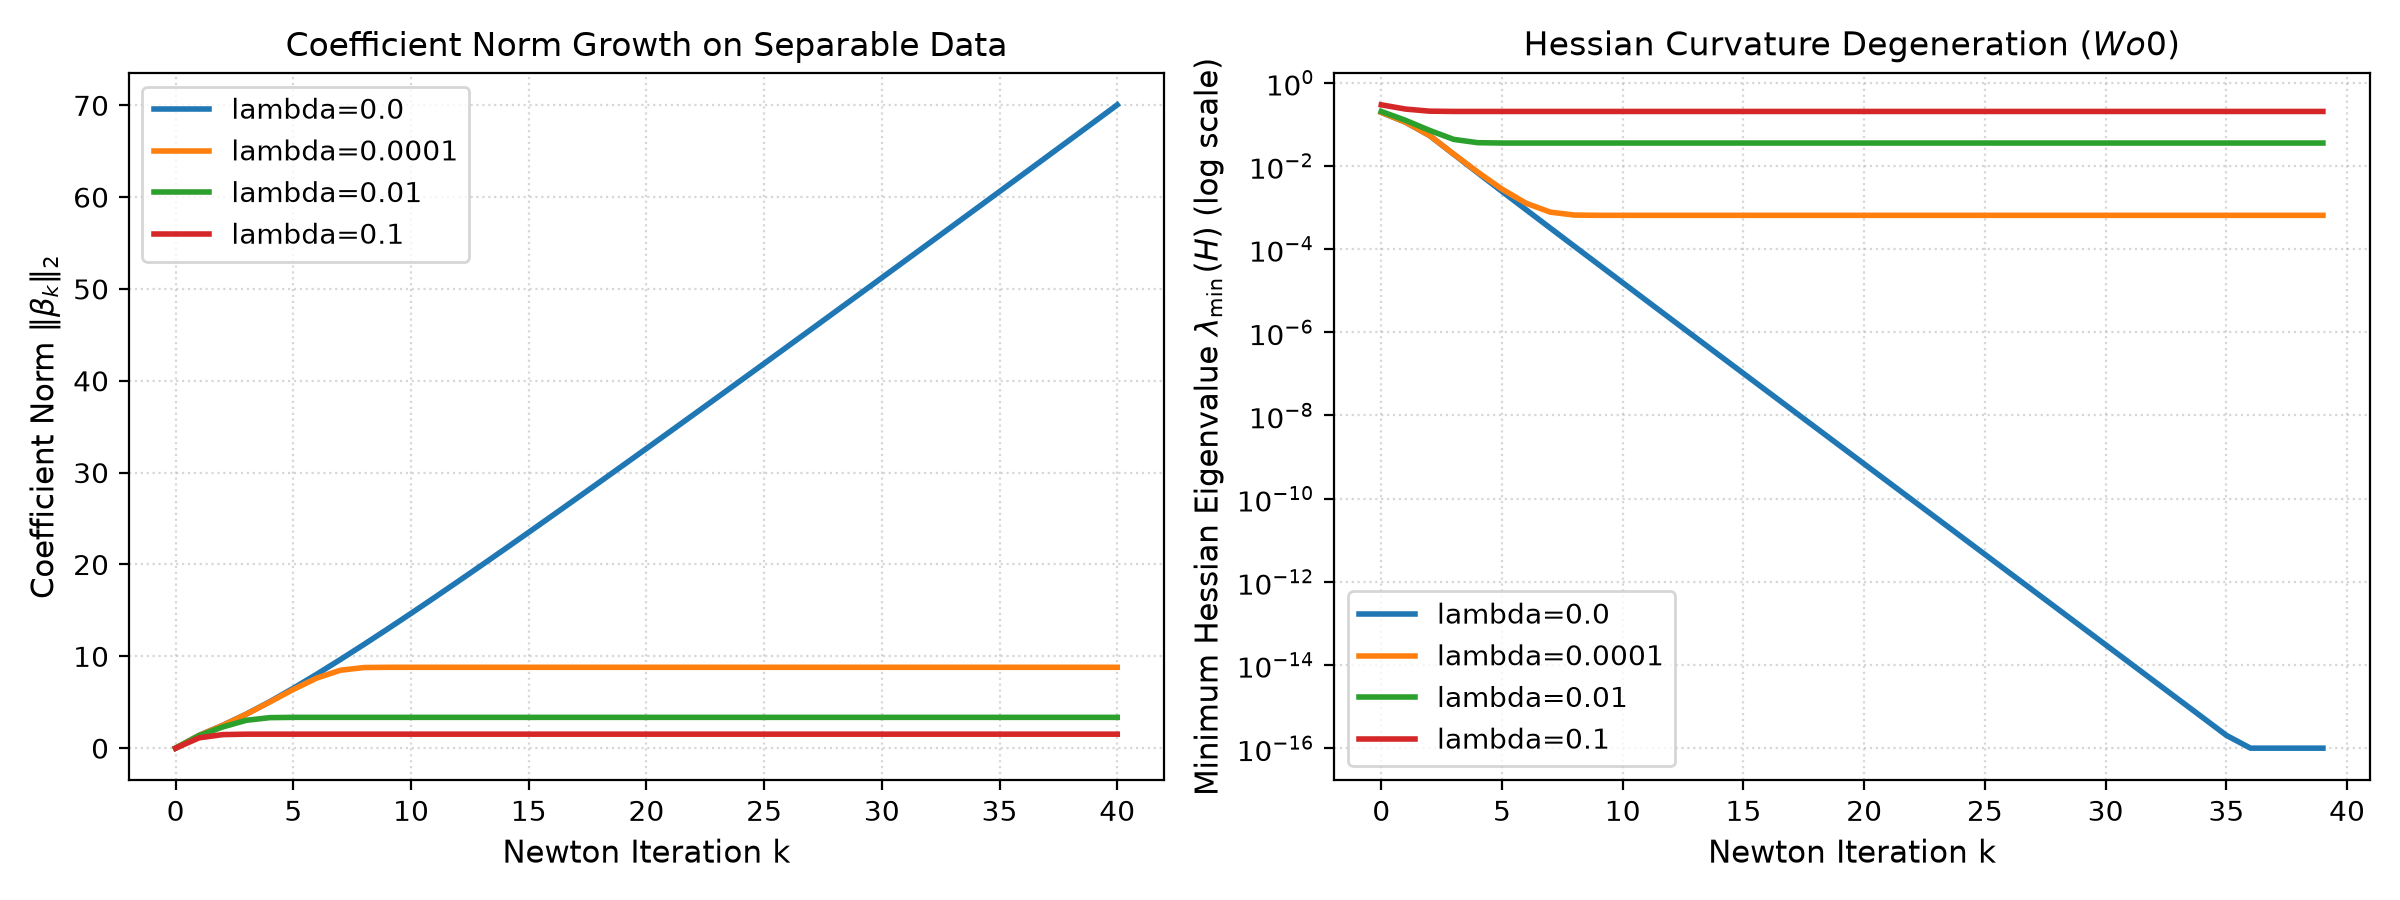
\includegraphics[width=0.88\linewidth]{experiment_e_separability.png}
\caption{Coefficient norm growth (left) and Hessian eigenvalue degeneration (right) on separable data.}\label{fig:exp_e}
\end{figure}

Adding an $\ell_2$ penalty ($\lambda = 10^{-4}$) strictly bounded coefficient growth ($\|\beta\|_2 = 8.81$) and guaranteed strict positive definiteness ($\lambda_{\min} \ge 6.44 \times 10^{-4} > 0$), restoring coercivity and guaranteeing a finite unique minimizer.

\section{Discussion and Practical Guidelines}
\begin{enumerate}
  \item \textbf{Small to Moderate Dimensionality ($p \lesssim 1000$):} Damped Newton's method is overwhelmingly superior in speed, robustness, and precision, converging in 5–15 iterations regardless of ill-conditioning or correlation.
  \item \textbf{High Dimensionality ($p \gg 1000$):} The $\mathcal{O}(np^2 + p^3)$ Hessian bottleneck becomes prohibitive. Limited-memory quasi-Newton methods (L-BFGS) provide the optimal balance, approximating second-order curvature with $\mathcal{O}(mp)$ memory.
  \item \textbf{Feature Normalization is Mandatory for First-Order Methods:} Disparate feature scales deform the loss landscape into severe anisotropic valleys that cripple first-order methods.
  \item \textbf{Always Apply $\ell_2$ Shrinkage:} Even a small regularizer ($\lambda = 10^{-4}$) prevents parameter blowup on linearly separable data and guarantees numerical well-posedness.
\end{enumerate}

\section{Conclusion}
Starting from the Bernoulli likelihood, this study developed from-first-principles derivations and implementations of first- and second-order logistic regression optimizers. Automated derivative testing confirmed analytical accuracy to $< 10^{-8}$ relative error. On the Wisconsin Diagnostic Breast Cancer dataset, damped Newton optimization matched gradient descent's regularized predictive performance while reducing iterations by $2,981\times$ and runtime by $965\times$. Controlled numerical experiments validated theoretical Lipschitz step-size bounds, demonstrated Newton's affine invariance and resilience to correlation, identified the cubic dimensionality complexity crossover, and proved the necessity of $\ell_2$ regularization for ensuring finite maximum likelihood estimates.

\section*{Reproducibility}
The complete codebase, test suite, and experimental pipelines are available in the repository. To reproduce all results and figures:
\begin{lstlisting}[language=bash]
# Run 40 automated unit tests:
python -m pytest tests/ -v

# Execute complete experimental pipeline:
PYTHONPATH=.:src python experiments/run_all.py --out results
\end{lstlisting}

\begin{thebibliography}{9}
\bibitem{nocedal2006} J. Nocedal and S. J. Wright, \emph{Numerical Optimization}, 2nd ed. Springer, 2006.
\bibitem{boyd2004} S. Boyd and L. Vandenberghe, \emph{Convex Optimization}. Cambridge University Press, 2004.
\bibitem{hastie2009} T. Hastie, R. Tibshirani, and J. Friedman, \emph{The Elements of Statistical Learning}, 2nd ed. Springer, 2009.
\bibitem{bishop2006} C. M. Bishop, \emph{Pattern Recognition and Machine Learning}. Springer, 2006.
\bibitem{sklearn} Scikit-learn developers, ``Breast cancer Wisconsin dataset,'' \emph{scikit-learn documentation}, 2024.
\end{thebibliography}

\end{document}
